% !TeX program = xelatex
%!TEX root = document.tex
% !TeX encoding = UTF-8

\documentclass[aspectratio=169, 10pt]{beamer}

% ============================================================
% IQB Beamer Theme
% ============================================================
\usepackage{../../../theme/beamerthemeiqb}
\usepackage{../../../theme/iqb-layouts}
\renewcommand{\iqbheaderimage}{../../../theme/images/header.png}
\setstretch{1.05}

\usepackage{amsmath}
\usepackage{amssymb}
\usepackage[version=4]{mhchem}
\usepackage{booktabs}
% Fix protein.png path for this subdirectory
\renewcommand{\iqbsectionframe}[2]{%
  \setsection{#1}%
  \begin{frame}[plain,noframenumbering]
    \begingroup
      % Hide footer on section divider
      \setbeamertemplate{footline}{}
      % Background gradient
      \begin{tikzpicture}[remember picture,overlay]
        \fill[white] (current page.south west) rectangle (current page.north east);
        \shade[left color=white, right color=iqblightgray!30]
              (current page.south west) rectangle (current page.north east);
      \end{tikzpicture}
      % Left vertical bar
      \begin{tikzpicture}[remember picture,overlay]
        \draw[line width=8pt, color=iqbblue]
             (current page.north west) -- (current page.south west);
      \end{tikzpicture}
      % Decorative protein (FIXED PATH)
      \begin{tikzpicture}[remember picture,overlay]
        \node[anchor=south east, inner sep=0pt, opacity=0.12]
             at ($(current page.south east) + (-1cm, 1cm)$) {
          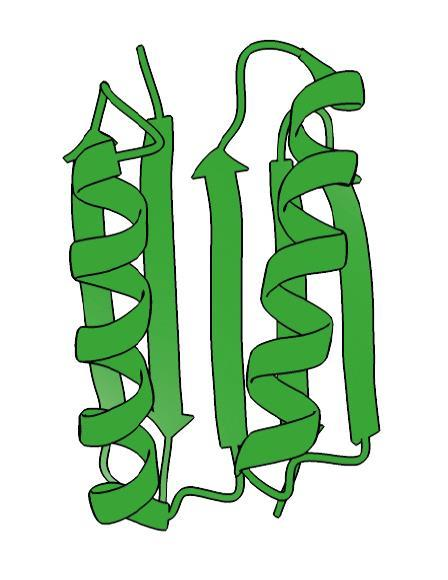
\includegraphics[height=5cm,keepaspectratio]{../../../theme/images/protein.png}
        };
      \end{tikzpicture}
      % Title
      \vspace*{0.5cm}
      \begin{center}
        {\Huge\color{iqbblue}\textbf{#2}}\\[0.3cm]
        {\Large\color{iqbgray}#1}
      \end{center}
      \vspace*{0.3cm}
    \endgroup
  \end{frame}
}

% 缩小子项缩进（本课程讲义使用更紧凑的层级）
\renewcommand{\subitem}[1]{%
  \par\vspace{2pt}%
  \noindent\hspace{0.8em}\textcolor{iqbblue}{$\circ$}\ #1%
}


% ============================================================
% Meta Information
% ============================================================
% 设置教材信息
\iqbtextbook{Quantum Chemistry}{Levine}{7th Edition}{Pearson}

% 课程讲义元数据
\lecturetitle{第三章：算符理论}
\lectureengtitle{Chapter 3: Operators, Algebra, and Eigenvalue Problems}

\author{东山月光下QM小组}
\date{\today}

% ============================================================
% Document Start
% ============================================================
\begin{document}

% ============================================================
% Title Frame
% ============================================================
\iqbcoverframe

% ============================================================
% Overview
% ============================================================
\begin{frame}{本章概览：算符理论的完整框架}
  \begin{iqbitemize}
    \item \textbf{算符基础}（Operator Basics）：定义、线性算符、常见算符实例
    \item \textbf{算符代数}（Operator Algebra）：加法、乘法、幂运算、算符函数
    \item \textbf{对易关系}（Commutation Relations）：对易子及其物理意义
    \item \textbf{本征值问题}（Eigenvalue Problems）：本征方程、可观测量、完备性
  \end{iqbitemize}

  \iqbbigsep

  \iqbgreenbox{核心思想}{算符是量子力学的语言，将物理量转化为数学对象}
\end{frame}

% ============================================================
% Section 3.1: Operators
% ============================================================
\iqbsectionframe{Section 3.1}{算符基础 (Operators)}

\begin{frame}{什么是算符？从薛定谔方程说起}

  
    \iqbsectiontitle[iqbgreen]{从薛定谔方程引入算符   }
  \begin{iqbitemize}
      \item \textbf{定态薛定谔方程}（time-independent Schrödinger equation）可以写成算符形式
      \[
        \left[-\dfrac{\hbar^2}{2m}\dfrac{\mathrm{d}^2}{\mathrm{d}x^2} + V(x)\right]\psi(x) = E\psi(x)
      \]
      \item 方括号内的整体是一个\textbf{算符}（operator），称为\textbf{哈密顿算符}（Hamiltonian operator）$\hat{H}$
      \item 算符作用在\textbf{波函数}（wave function）$\psi(x)$上，产生同样的波函数乘以能量$E$
      \item 这启示我们：算符是量子力学描述物理量的数学语言
    \end{iqbitemize}

    \iqbtinysep

    \iqbsectiontitle[iqbgreen]{算符的直观理解}
    \begin{iqbitemize}
      \item 算符是一个\textbf{操作规则}或\textbf{变换指令}
      \item 它接受一个函数作为输入，输出另一个函数
      \item 就像机器：输入原料（函数）→ 加工处理 → 输出产品（新函数）
      \item 用帽子符号$\hat{\ }$标记算符，以区别于普通数字
    \end{iqbitemize}
    \iqbsectiontitle[iqbgreen]{具体例子}
    \begin{iqbitemize}
      \item \textbf{微分算符}（differential operator）$\hat{D} = \dfrac{\mathrm{d}}{\mathrm{d}x}$
      \[
        \hat{D}(x^2 + 3e^{2x}) = 2x + 6e^{2x}
      \]
      对原函数求导，得到新函数

      \item \textbf{乘法算符}$\hat{3}$（乘以3）
      \[
        \hat{3}(x + e^{x}) = 3x + 3e^{x}
      \]
      将原函数整体乘以3

      \item \textbf{三角算符}$\hat{T}$：
      \[
        \hat{T}f(x) = \tan[f(x)]
      \]
      对函数取正切
    \end{iqbitemize}

    \iqborangebox{核心概念}{算符不是数值而是对函数进行变换的操作或规则}
  }
\end{frame}


      \item \textbf{例子}：设$\hat{D} = \dfrac{\mathrm{d}}{\mathrm{d}x}$，$\hat{3}$为乘以3
      \[
        (\hat{D} + \hat{3})(x^3 - 5x) = \hat{D}(x^3 - 5x) + \hat{3}(x^3 - 5x)
      \]
      \[
        = (3x^2 - 5) + (3x^3 - 15x) = 3x^3 + 3x^2 - 15x - 5
      \]

      \item 算符加法满足\textbf{交换律}：$\hat{A} + \hat{B} = \hat{B} + \hat{A}$

      \item 算符加法满足\textbf{结合律}：$(\hat{A} + \hat{B}) + \hat{C} = \hat{A} + (\hat{B} + \hat{C})$
% \end{iqbitemize}
    \end{iqbitemize}
    \iqbsectiontitle[iqbgreen]{算符的乘积}
    \begin{iqbitemize}
      \item \textbf{关键规则}：从右向左依次作用
      \[
        \hat{A}\hat{B}f(x) = \hat{A}[\hat{B}f(x)]
      \]
      先作用右边的$\hat{B}$，再对结果作用左边的$\hat{A}$

      \item \textbf{例子}：$\hat{3}\hat{D}f(x)$
      \[
        \hat{3}\hat{D}f(x) = \hat{3}[\hat{D}f(x)] = \hat{3}[f'(x)] = 3f'(x)
      \]
      先求导，再乘以3

      \item \textbf{重要}：算符乘法\textbf{一般不满足交换律}
      \[
        \hat{A}\hat{B} \neq \hat{B}\hat{A}
      \]
      顺序不同，结果可能不同

      \item 这是量子力学与经典力学的\textbf{根本区别}
    \end{iqbitemize}

    \iqbgreenbox{核心}{算符乘积的顺序至关重要，这是\textbf{对易关系}（commutation relation）的起源}
\end{frame}

\begin{frame}{算符等式与代数规则}
  
    \iqbsectiontitle[iqbgreen]{算符相等的严格定义   }
  \begin{iqbitemize}
    \item \textbf{数学定义}（operator equality）
    \end{iqbitemize}
      \[
        \hat{A} = \hat{B} \quad \text{当且仅当} \quad \hat{A}f = \hat{B}f \quad \text{对所有函数}f
      \]
    \begin{iqbitemize}
    \item 两算符相等意味着对任意函数的作用结果相同
    \item \textbf{常见错误}：不能仅从一次作用就判断算符相等
    \end{iqbitemize}
      \[
        \frac{d}{dx}e^{2x} = 2e^{2x} \quad \text{但} \quad \frac{d}{dx} \neq 2
      \]
    \begin{iqbitemize}
    \item 因为等式不对所有函数成立（例如对$x^2$不成立）
    \end{iqbitemize}
    \iqbsectiontitle[iqbgreen]{算符代数的基本规则}
    \begin{iqbitemize}
    \item \textbf{结合律}（associative）：
    \[
      (\hat{A}\hat{B})\hat{C} = \hat{A}(\hat{B}\hat{C})
    \]
    \item \textbf{分配律}（distributive）：
    \[
      \hat{A}(\hat{B} + \hat{C}) = \hat{A}\hat{B} + \hat{A}\hat{C}
    \]
    \item \textbf{交换律不成立}（non-commutative）：
    \[
      \hat{A}\hat{B} \neq \hat{B}\hat{A} \quad \text{（一般情况）}
    \]
    \item 这是算符代数与普通代数的\textbf{根本区别}
    \end{iqbitemize}
    \iqbtinysep

    \iqbgreenbox{关键洞察}{算符乘法顺序影响结果，体现量子力学的本质特征}
\end{frame}

\begin{frame}{算符等式的推导：对易关系的起源}
  
    \iqbsectiontitle[iqbgreen]{推导目标   }
  \begin{iqbitemize}
    \item 证明微分算符与乘法算符的重要关系：
    \end{iqbitemize}
      \[
        \boxed{\hat{D}\hat{x} = \hat{1} + \hat{x}\hat{D}}
      \]
    \begin{iqbitemize}
    \item \textbf{方法}：利用算符相等定义，证明两边对任意函数$f(x)$作用结果相同
    \end{iqbitemize}
    \iqbtinysep

    \iqbsectiontitle[iqbgreen]{左边作用：$\hat{D}\hat{x}f(x)$}
    \begin{iqbitemize}
    \item 计算：$\dfrac{\mathrm{d}}{\mathrm{d}x}[xf(x)]$
    \item 使用乘积求导法则：$(uv)' = u'v + uv'$
    \end{iqbitemize}
      \[
        \dfrac{\mathrm{d}}{\mathrm{d}x}[xf(x)] = 1 \cdot f(x) + x \cdot f'(x) = f(x) + x\dfrac{\mathrm{d}f}{\mathrm{d}x}
      \]
    \iqbsectiontitle[iqbgreen]{右边作用：$(\hat{1} + \hat{x}\hat{D})f(x)$}
    \begin{iqbitemize}
    \item 计算：$\hat{1}f(x) + \hat{x}\hat{D}f(x)$
    \end{iqbitemize}
      \[
        f(x) + x\dfrac{\mathrm{d}f}{\mathrm{d}x}
      \]
    \begin{iqbitemize}
    \item 与左边结果\textbf{完全相同}
    \end{iqbitemize}
    \iqbsmallsep

    \iqbsectiontitle[iqbgreen]{关键结论}
    \begin{iqbitemize}
    \item $\hat{D}\hat{x} - \hat{x}\hat{D} = \hat{1}$
    \item 定义对易子：$[\hat{D}, \hat{x}] = \hat{D}\hat{x} - \hat{x}\hat{D} = \hat{1}$
    \item 这是\textbf{海森堡不确定性原理}的数学基础
    \end{iqbitemize}
    \iqbtinysep

    \iqbgreenbox{物理意义}{位置算符与动量算符不可对易，导致位置和动量不能同时精确测量}
\end{frame}

\begin{frame}{算符的线性：为什么如此重要？}
  
  
    \iqbsectiontitle[iqbgreen]{线性算符的直观理解   }
  \begin{iqbitemize}
      \item \textbf{叠加性的物理意义}
      \begin{itemize}
        \setlength{\itemsep}{0.05cm}
        \item 如果系统可以处于状态$\psi_1$或$\psi_2$
        \item 那么也可以处于它们的\textbf{线性组合}（linear combination）$c_1\psi_1 + c_2\psi_2$
        \item 这是\textbf{量子叠加原理}（quantum superposition principle）的数学表达
      \end{itemize}

      \item \textbf{齐次性的物理意义}
      \begin{itemize}
        \setlength{\itemsep}{0.05cm}
        \item 将波函数整体放大或缩小$c$倍
        \item 不改变系统的物理状态
        \item 因为概率密度$|\psi|^2$会相应缩放，但归一化条件保持比例
      \end{itemize}

      \item \textbf{为什么量子力学算符必须是线性的？}
      \begin{itemize}
        \setlength{\itemsep}{0.05cm}
        \item 实验观察：量子态满足叠加原理
        \item 数学要求：薛定谔方程是\textbf{线性微分方程}（linear differential equation）
        \item 物理后果：保证概率诠释的一致性
      \end{itemize}
    \end{iqbitemize}
    \iqbsectiontitle[iqbgreen]{线性的数学验证}
    \begin{iqbitemize}
      \item \textbf{验证拉普拉斯算符的线性}
      \[
        \nabla^2 = \dfrac{\partial^2}{\partial x^2} + \dfrac{\partial^2}{\partial y^2} + \dfrac{\partial^2}{\partial z^2}
      \]

      \item \textbf{叠加性验证}
      \begin{align*}
        \nabla^2(f+g) &= \dfrac{\partial^2(f+g)}{\partial x^2} + \cdots \\
                  &= \dfrac{\partial^2 f}{\partial x^2} + \dfrac{\partial^2 g}{\partial x^2} + \cdots \\
                  &= \nabla^2 f + \nabla^2 g
      \end{align*}

      \item \textbf{齐次性验证}
      \begin{align*}
        \nabla^2(cf) &= \dfrac{\partial^2(cf)}{\partial x^2} + \cdots \\
                 &= c\dfrac{\partial^2 f}{\partial x^2} + \cdots \\
                 &= c\nabla^2 f
      \end{align*}

      \item \textbf{非线性的反例}
      \[
        \sqrt{\hat{\ }}f(x) = \sqrt{f(x)}
      \]
      显然$\sqrt{f+g} \neq \sqrt{f} + \sqrt{g}$，不满足线性
    \end{iqbitemize}
  }
\end{frame}

\begin{frame}{线性算符（1/2）：定义与条件}

  
    \iqbsectiontitle[iqbgreen]{线性算符的定义   }
  \begin{iqbitemize}
    \item 算符$\hat{A}$是线性的，当且仅当满足两个条件
    \end{iqbitemize}

    \iqborangebox{定义}{线性是量子力学算符的核心性质}
    \iqbsectiontitle[iqbgreen]{条件1：叠加性}
    \begin{iqbitemize}
    \item 数学表达：
    \end{iqbitemize}
      \[
        \hat{A}[f(x) + g(x)] = \hat{A}f(x) + \hat{A}g(x)
      \]
    \begin{iqbitemize}
    \item 物理意义：两个函数之和的算符作用等于各函数算符作用之和
    \item 这允许我们将复杂状态分解为简单状态的叠加
    \end{iqbitemize}

    \iqbgreenbox{叠加性}{可分解性}
\end{frame}

\begin{frame}{线性算符（2/2）：齐次性与应用}

  
    \iqbsectiontitle[iqbgreen]{条件2：齐次性   }
  \begin{iqbitemize}
    \item 数学表达：
    \end{iqbitemize}
      \[
        \hat{A}[c \cdot f(x)] = c \cdot \hat{A}f(x)
      \]
    \begin{iqbitemize}
    \item 物理意义：常数倍函数的算符作用等于常数倍的算符作用
    \item 确保算符作用保持波函数的归一化性质
    \end{iqbitemize}

    \iqborangebox{齐次性}{标量不变性}
    \iqbsectiontitle[iqbgreen]{为什么需要线性算符？}
    \begin{iqbitemize}
    \item \textbf{叠加原理的数学基础}：
    \subitem{量子系统可处于多个状态的叠加}
    \subitem{例如：$\Psi = c_1\psi_1 + c_2\psi_2$}

    \item \textbf{态的线性演化}：
    \subitem{薛定谔方程是线性的}
    \subitem{初始态的线性叠加演化为末态的线性叠加}

    \item \textbf{测量理论的要求}：
    \subitem{本征函数构成完备集}
    \subitem{任意态可展开为本征态的叠加}
    \end{iqbitemize}

    \iqbgreenbox{关键}{线性确保量子态演化保持幺正性}
\end{frame}

\begin{frame}{线性算符实例}

  \iqbsectiontitle[iqbgreen]{常见线性算符}

  \begin{iqbitemize}
  \item \textbf{微分算符}：
  \[
    \hat{D} = \dfrac{\mathrm{d}}{\mathrm{d}x}
  \]
  \subitem{作用：求函数的导数}

  \item \textbf{Laplace算符}：
  \[
    \nabla^2 = \dfrac{\partial^2}{\partial x^2} + \dfrac{\partial^2}{\partial y^2} + \dfrac{\partial^2}{\partial z^2}
  \]
  \subitem{作用：求二阶导数，描述动能项}

  \item \textbf{哈密顿算符}：
  \[
    \hat{H} = -\dfrac{\hbar^2}{2m}\nabla^2 + V(x,y,z)
  \]
  \subitem{作用：给出系统的总能量}

  \item \textbf{乘法算符}：
  \[
    \hat{x}, \quad \hat{p}_x = -i\hbar\dfrac{\partial}{\partial x}, \quad \hat{V}(x)
  \]
  \subitem{作用：坐标、动量、势能算符}
  \end{iqbitemize}

  \iqbsep

  \iqbgreenbox{核心}{所有量子力学算符都是线性算符}
\end{frame}

\begin{frame}{算符代数：乘法顺序至关重要}
  
  
    \iqbsectiontitle[iqbgreen]{算符的加减   }
  \begin{iqbitemize}
      \item 两个算符之和定义为：
      \[
        (\hat{A} + \hat{B})f(x) = \hat{A}f(x) + \hat{B}f(x)
      \]
      \item 两个算符之差定义为：
      \[
        (\hat{A} - \hat{B})f(x) = \hat{A}f(x) - \hat{B}f(x)
      \]
      \item 算符加减后仍是算符
      \item 加法满足交换律：$\hat{A} + \hat{B} = \hat{B} + \hat{A}$
    \end{iqbitemize}
    \iqbsectiontitle[iqbgreen]{算符的乘积}
    \begin{iqbitemize}
      \item 算符乘积定义为连续作用：
      \[
        \hat{A}\hat{B}f(x) = \hat{A}[\hat{B}f(x)]
      \]
      \item 先作用右边的算符$\hat{B}$，再作用左边的算符$\hat{A}$

      \iqbtinysep

      \item \textbf{重要}：算符乘法一般\textbf{不满足交换律}
      \[
        \hat{A}\hat{B} \neq \hat{B}\hat{A}
      \]

      \iqbtinysep

      \item 这是量子力学与经典力学的重要区别
    \end{iqbitemize}
  }
\end{frame}

\begin{frame}{验证算符线性：叠加原理的数学证明}
  
    \iqbsectiontitle[iqbgreen]{问题设定   }
  \begin{iqbitemize}
    \item 设$\hat{A} = \dfrac{\mathrm{d}}{\mathrm{d}x}$，$\hat{B} = x$
    \item 计算$\hat{A}\hat{B}$和$\hat{B}\hat{A}$并比较
    \end{iqbitemize}
    \iqbsmallsep

    \iqbsectiontitle[iqbgreen]{计算$\hat{A}\hat{B}f(x)$}
    \begin{iqbitemize}
    \item 先乘法后求导：
    \end{iqbitemize}
      \[
        \hat{A}\hat{B}f(x) = \dfrac{\mathrm{d}}{\mathrm{d}x}[x f(x)] = f(x) + x f'(x)
      \]
    \iqbsectiontitle[iqbgreen]{计算$\hat{B}\hat{A}f(x)$}
    \begin{iqbitemize}
    \item 先求导后乘法：
    \end{iqbitemize}
      \[
        \hat{B}\hat{A}f(x) = x \cdot \dfrac{\mathrm{d}}{\mathrm{d}x}f(x) = x f'(x)
      \]
    \iqbsmallsep

    \iqbsectiontitle[iqbgreen]{结论}
    \begin{iqbitemize}
    \item $\hat{A}\hat{B} - \hat{B}\hat{A} = \hat{1}$
    \item 对易子：$[\hat{A}, \hat{B}] = \hat{1}$
    \end{iqbitemize}

    \iqbgreenbox{关键}{算符顺序改变结果，量子力学本质特征}
\end{frame}

% ============================================================
% Example 3.1: Operator Algebra
% ============================================================
\begin{frame}{例题3.1：验证算符代数恒等式}
  
  \iqbsectiontitle[iqbgreen]{验证$(\hat{A} + \hat{B})^2 \neq \hat{A}^2 + 2\hat{A}\hat{B} + \hat{B}^2$}

  \textbf{问题}：设$\hat{A} = \dfrac{\mathrm{d}}{\mathrm{d}x}$，$\hat{B} = x$，验证算符平方展开

  \iqbsep

  \begin{iqbitemize}
    \item \textbf{经典代数}：$(a+b)^2 = a^2 + 2ab + b^2$

    \item \textbf{算符代数}：一般\textcolor{red}{不成立}！
    \[
      (\hat{A} + \hat{B})^2 = (\hat{A} + \hat{B})(\hat{A} + \hat{B}) = \hat{A}^2 + \hat{A}\hat{B} + \hat{B}\hat{A} + \hat{B}^2
    \]

    \item \textbf{验证}：左边$(\hat{D} + \hat{x})^2 = (\hat{D} + \hat{x})(\hat{D} + \hat{x})$
    \begin{align*}
      &= \hat{D}^2 + \hat{D}\hat{x} + \hat{x}\hat{D} + \hat{x}^2 \\
      &= \hat{D}^2 + (\hat{1} + \hat{x}\hat{D}) + \hat{x}\hat{D} + \hat{x}^2 \\
      &= \hat{D}^2 + \hat{1} + 2\hat{x}\hat{D} + \hat{x}^2
    \end{align*}

    \item \textbf{右边}：$\hat{A}^2 + 2\hat{A}\hat{B} + \hat{B}^2 = \hat{D}^2 + 2\hat{D}\hat{x} + \hat{x}^2$

    \item \textbf{比较}：
    \begin{itemize}
      \setlength{\itemsep}{0.05cm}
      \item 左边展开：$\hat{D}^2 + \hat{1} + 2\hat{x}\hat{D} + \hat{x}^2$
      \item 右边展开：$\hat{D}^2 + 2\hat{D}\hat{x} + \hat{x}^2$
      \item 差值：$\hat{1} + 2\hat{x}\hat{D} - 2\hat{D}\hat{x}$
      \item 由于$2\hat{x}\hat{D} \neq 2\hat{D}\hat{x}$，两边不相等
    \end{itemize}
  \end{iqbitemize}

  \iqbgreenbox{结论}{算符代数必须严格按照定义展开，不能套用经典代数公式}
\end{frame}

\begin{frame}{例题3.2：算符多项式的计算}
  
  \iqbsectiontitle[iqbgreen]{计算$(\hat{A}+\hat{B})^3$的展开式}

  \textbf{问题}：展开算符多项式$(\hat{A}+\hat{B})^3$并说明需要注意的问题

  \iqbsep

  \begin{iqbitemize}
    \item \textbf{错误的展开}（套用经典代数）：
    \[
      (\hat{A}+\hat{B})^3 \neq \hat{A}^3 + 3\hat{A}^2\hat{B} + 3\hat{A}\hat{B}^2 + \hat{B}^3
    \]

    \item \textbf{正确的展开}（保持算符顺序）：
    \begin{align*}
      (\hat{A}+\hat{B})^3 &= (\hat{A}+\hat{B})(\hat{A}+\hat{B})(\hat{A}+\hat{B}) \\
      &= (\hat{A}+\hat{B})(\hat{A}^2 + \hat{A}\hat{B} + \hat{B}\hat{A} + \hat{B}^2) \\
      &= \hat{A}^3 + \hat{A}^2\hat{B} + \hat{A}\hat{B}\hat{A} + \hat{A}\hat{B}^2 \\
      &\quad + \hat{B}\hat{A}^2 + \hat{B}\hat{A}\hat{B} + \hat{B}^2\hat{A} + \hat{B}^3
    \end{align*}

    \item \textbf{关键区别}：
    \begin{itemize}
      \setlength{\itemsep}{0.05cm}
      \item 经典：乘法可交换，$a^2b = ab^2$
      \item 算符：$\hat{A}^2\hat{B} \neq \hat{A}\hat{B}\hat{A}$，顺序重要
      \item 所有8项都代表不同作用顺序，不能合并
    \end{itemize}

    \item \textbf{特例}：若$[\hat{A},\hat{B}]=0$则可交换
  \end{iqbitemize}

  \iqbgreenbox{关键}{算符乘法必须保持顺序}
\end{frame}

% ============================================================
% Section 3.2: Operator Algebra
% ============================================================
\iqbsectionframe{Section 3.2}{算符代数 (Operator Algebra)}

\begin{frame}{算符的幂运算}
  
  
    \iqbsectiontitle[iqbgreen]{定义与性质   }
  \begin{iqbitemize}
      \item 算符的$n$次幂定义为连续作用$n$次
      \[
        \hat{A}^n f(x) = \underbrace{\hat{A}\hat{A}\cdots\hat{A}}_{n\text{次}}f(x)
      \]

      \item 例如：$(\dfrac{\mathrm{d}}{\mathrm{d}x})^2 f(x) = \dfrac{\mathrm{d}^2f}{\mathrm{d}x^2}$

      \item 指数律成立：$\hat{A}^m \hat{A}^n = \hat{A}^{m+n}$

      \item 算符函数可用幂级数定义
      \[
        e^{\hat{A}} = \hat{1} + \hat{A} + \dfrac{\hat{A}^2}{2!} + \dfrac{\hat{A}^3}{3!} + \cdots
      \]
    \end{iqbitemize}
    \iqbsectiontitle[iqbgreen]{实际应用}
    \begin{iqbitemize}
      \item \textbf{动能算符}：
      \[
        \hat{T} = -\dfrac{\hbar^2}{2m}\dfrac{\mathrm{d}^2}{\mathrm{d}x^2}
      \]
      涉及二阶导数算符

      \item \textbf{哈密顿算符}：
      \[
        \hat{H} = \hat{T} + \hat{V}
      \]
      动能算符与势能算符之和

      \item \textbf{平移算符}：
      \[
        e^{a\dfrac{\mathrm{d}}{\mathrm{d}x}}f(x) = f(x+a)
      \]
      指数算符产生函数平移
    \end{iqbitemize}

    \iqbtinysep

    \iqborangebox{注意}{算符函数的级数展开必须收敛才有意义}
  }
\end{frame}

\begin{frame}{算符多项式与函数}
  
  
    \iqbsectiontitle[iqbgreen]{算符多项式的定义   }
  \begin{iqbitemize}
    \item 算符多项式是算符幂的线性组合
    \end{iqbitemize}
      \[
        P(\hat{A}) = c_0\hat{1} + c_1\hat{A} + c_2\hat{A}^2 + \cdots + c_n\hat{A}^n
      \]
    \begin{iqbitemize}
    \item \textbf{单算符多项式}：类似普通代数
    \[
      (\hat{A} + \hat{1})^2 = \hat{A}^2 + 2\hat{A} + \hat{1}
    \]
    \item 因为算符与自身对易：$[\hat{A}, \hat{A}] = 0$
    \end{iqbitemize}
    \iqbsmallsep

    \iqbsectiontitle[iqbgreen]{双算符多项式的复杂性}
    \begin{iqbitemize}
    \item \textbf{常见错误}：
    \[
      (\hat{A} + \hat{B})^2 \neq \hat{A}^2 + 2\hat{A}\hat{B} + \hat{B}^2
    \]
    \item 原因：$\hat{A}$与$\hat{B}$不对易
    \end{iqbitemize}
    \iqbtinysep

    \iqbsectiontitle[iqbgreen]{正确展开方式}
    \begin{iqbitemize}
    \item 保留算符顺序：
    \[
      (\hat{A} + \hat{B})^2 = \hat{A}^2 + \hat{A}\hat{B} + \hat{B}\hat{A} + \hat{B}^2
    \]
    \item 使用对易子简化：
    \[
      (\hat{A} + \hat{B})^2 = \hat{A}^2 + 2\hat{A}\hat{B} + \hat{B}^2 + [\hat{B}, \hat{A}]
    \]
    \end{iqbitemize}
    \iqbsectiontitle[iqbgreen]{算符函数的定义}
    \begin{iqbitemize}
    \item 通过\textbf{泰勒级数展开}（Taylor series）定义
    \[
      f(\hat{A}) = \sum_{n=0}^{\infty} \dfrac{f^{(n)}(0)}{n!}\hat{A}^n
    \]
    \item \textbf{指数算符}（exponential operator）：
    \end{iqbitemize}
      \[
        e^{\hat{A}} = \hat{1} + \hat{A} + \dfrac{1}{2!}\hat{A}^2 + \dfrac{1}{3!}\hat{A}^3 + \cdots
      \]
    \begin{iqbitemize}
    \item 物理中的重要应用：
    \subitem{时间演化算符：$e^{-i\hat{H}t/\hbar}$}
    \subitem{平移算符：$e^{a\mathrm{d}/\mathrm{d}x}$}
    \subitem{旋转算符：$e^{-i\hat{L}_z\phi/\hbar}$}
    \end{iqbitemize}
    \iqbsmallsep

    \iqbsectiontitle[iqbgreen]{算符函数的性质}
    \begin{iqbitemize}
    \item 级数必须收敛才有意义
    \item 若$[\hat{A}, \hat{B}] = 0$，则$e^{\hat{A}}e^{\hat{B}} = e^{\hat{A}+\hat{B}}$
    \item 一般情况需用Baker-Campbell-Hausdorff公式
    \end{iqbitemize}

    \iqbgreenbox{物理意义}{算符函数描述量子态的演化}
\end{frame}

\end{document}
